%% V1.0
%% by Gabriel Garcia, gabrcg@gmail.com
%% This is a template for Udacity projects using IEEEtran.cls

%% Be Udacious!

\documentclass[10pt,journal,compsoc]{IEEEtran}

\usepackage[pdftex]{graphicx}    
\usepackage{cite}
\hyphenation{op-tical net-works semi-conduc-tor}


\begin{document}

\title{Deep RL Arm Manipulation}

\author{Saminda Abeyruwan}

\markboth{Deep RL Arm Manipulation}%
{}
\IEEEtitleabstractindextext{%

\begin{abstract}

Deep reinforcement learning has enabled robotic systems to learn control or predictive  policies directly from camera inputs and raw pixels. In this project,  a simulated 3 degree-of-freedom robotic arm is trained to reach and touch an object of interest using a deep \textit{Q}-network. We have simulated two tasks, and show that the robot is successfully leaned the abilities to complete the scenarios.  
\end{abstract}

% Note that keywords are not normally used for peerreview papers.
\begin{IEEEkeywords}
Robot, IEEEtran, Udacity, \LaTeX, Deep RL, LSTM.
\end{IEEEkeywords}}


\maketitle
\IEEEdisplaynontitleabstractindextext
\IEEEpeerreviewmaketitle
\section{Introduction}
\label{sec:introduction}

\IEEEPARstart{D}{eep} reinforcement learning algorithms have been successfully applied to wide range of robotic control tasks, e.g., locomotion, robotic arm manipulation, and autonomous vehicle control \cite{GuHolLilLev17}. With the development of the deep \textit{Q}-networks and its variants  \cite{mnih2015humanlevel} \cite{Mnih:2016:AMD:3045390.3045594} \cite{Arulkumaran2017ABS}, the reinforcement learning paradigm has been scale to problems that were previously deemed intractable, e.g., learning to play video games from direct raw pixels.  

In this project, we have used an LSTM based deep \textit{Q}-network, similar to presented in \cite{DBLP:conf/aaaifs/HausknechtS15}, on 3 degree-of-freedom (DoF) robotic manipulator arm to reach and touch an object of interest in two scenarios:

\begin{enumerate}
\item have any part of the robot arm touch the object of interest, with at least a 90\% accuracy for a minimum of 100 runs, and
\item have only the gripper base of the robot arm touch the object, with at least a 80\% accuracy for a minimum of 100 runs.
\end{enumerate} 

The robot and the two tasks have been simulated in Gazebo \cite{288}, and we show that the robot is successfully leaned the abilities to complete the tasks with the given project requirements. 


%example for inserting image
%\begin{figure}[thpb]
%      \centering
%      \includegraphics[width=\linewidth]{RobotRevolution5}
%      \caption{Robot Revolution.}
%      \label{fig:robot1}
%\end{figure}

%\subsection{Subsection Heading Here}
%Subsection text here.
%
%\subsubsection{Subsubsection Heading Here}
%Subsubsection text here.
%
%
%\begin{table}[h]
%\caption{Table}
%\label{table_example}
%\begin{center}
%\begin{tabular}{|c||c|}
%\hline
%One & Two\\
%\hline
%Three & Four\\
%\hline
%\end{tabular}
%\end{center}
%\end{table}



   

\section{Reward Functions}

The first task requests to have any part of the robot arm touch the object of interest. The following reward structure has been used:

\begin{enumerate}
\item any part of the robot touches the object with reward +500.
\item any part of the robot, including gripper, collides with ground or itself, the reward has been set to -500.
\item an interim reward based on smoothed moving average. This function is composed of two parts:
\begin{enumerate}
\item For the time step $t$ and $t+1$, lets assume the robot gripper has incrementally moved $\delta_t=d_t - d_{t+1}$ distance, where, $d_t$ is the distance to the object from gripper.  If $\delta_t > 0$, it is an indication of the gripper moved closer to the object. Lets assume $\bar{\delta_t}$ is the moving average of $\delta_t$ distances. Then, we use the smoothing formula, $\bar{\delta}_{t+1} = \bar{\delta_{t}}\times \alpha + \delta_t \times (1 -  \alpha)$, where $\alpha \in [0, 1]$.
\item In order to encode the objective of completing the task as soon as possible, we have introduced a time step penalty, $time\_penalty$. This penalty has eliminate the gripper oscillating near the object of interest.  
\end{enumerate} Hence, using the prior decomposition, each step we have provided the reward $\bar{\delta_t} - time\_penalty$.  
\end{enumerate}

For the second task, we have used the following reward structure:

\begin{enumerate}
\item Only gripper touches the object with +500.
\item Any other collision resulted in a reward of -50. 
\item Similar to the first task, an interim reward based on smoothed moving average use been used. 
\end{enumerate}

%
%%example for Bullet point list
%
%\begin{itemize}
%\item example
%\end {itemize}
%
%
%
%%example for numbered list
%\begin{enumerate}
%\item example
%
%\end{enumerate}

\section{Hyperparameters}

We have used images of size $64 \times 64 \times 3$. The \textit{RMSprop} optimizer has been used in both tasks, while setting the learning rate to $0.1$. Neither tasks required changing the learning rate. We set the replay memory $10000$, and a batch size of $32$ has been used. We have enabled the LSTM mode, and the LSTM size has been set to $512$. The exploration rate, $\gamma$, has been set to $0.9$ and annihilated to $0.05$ over $200$ steps. We have used position control method to control the arm. Please refer to the definitions, $\mathsf{INPUT\_WIDTH}$, $\mathsf{INPUT\_HEIGHT}$, $\mathsf{OPTIMIZER}$, $\mathsf{LEARNING\_RATE}$, $\mathsf{REPLAY\_MEMORY}$, $\mathsf{BATCH\_SIZE}$, $\mathsf{USE\_LSTM}$, $\mathsf{LSTM\_SIZE}$,  $\mathsf{GAMMA}$, $\mathsf{EPS\_START}$, $\mathsf{EPS\_END}$, $\mathsf{EPS\_DECAY}$, and $\mathsf{VELOCITY\_CONTROL}$, in the associated code for the value binding.  

\section{Results}

The robot has learned successful control policies for both tasks within 200 episodes. We have let the first task, Fig. \ref{fig:task1}, to train over 600 episodes to reach 99\% of local accuracy. An instance of the completed second tasks is shown in Fig. \ref{fig:task2}. Both tasks were simulated using the same set of parameters.  Both tasks were completed using position based control. 

\begin{figure*}[thpb]
      \centering
      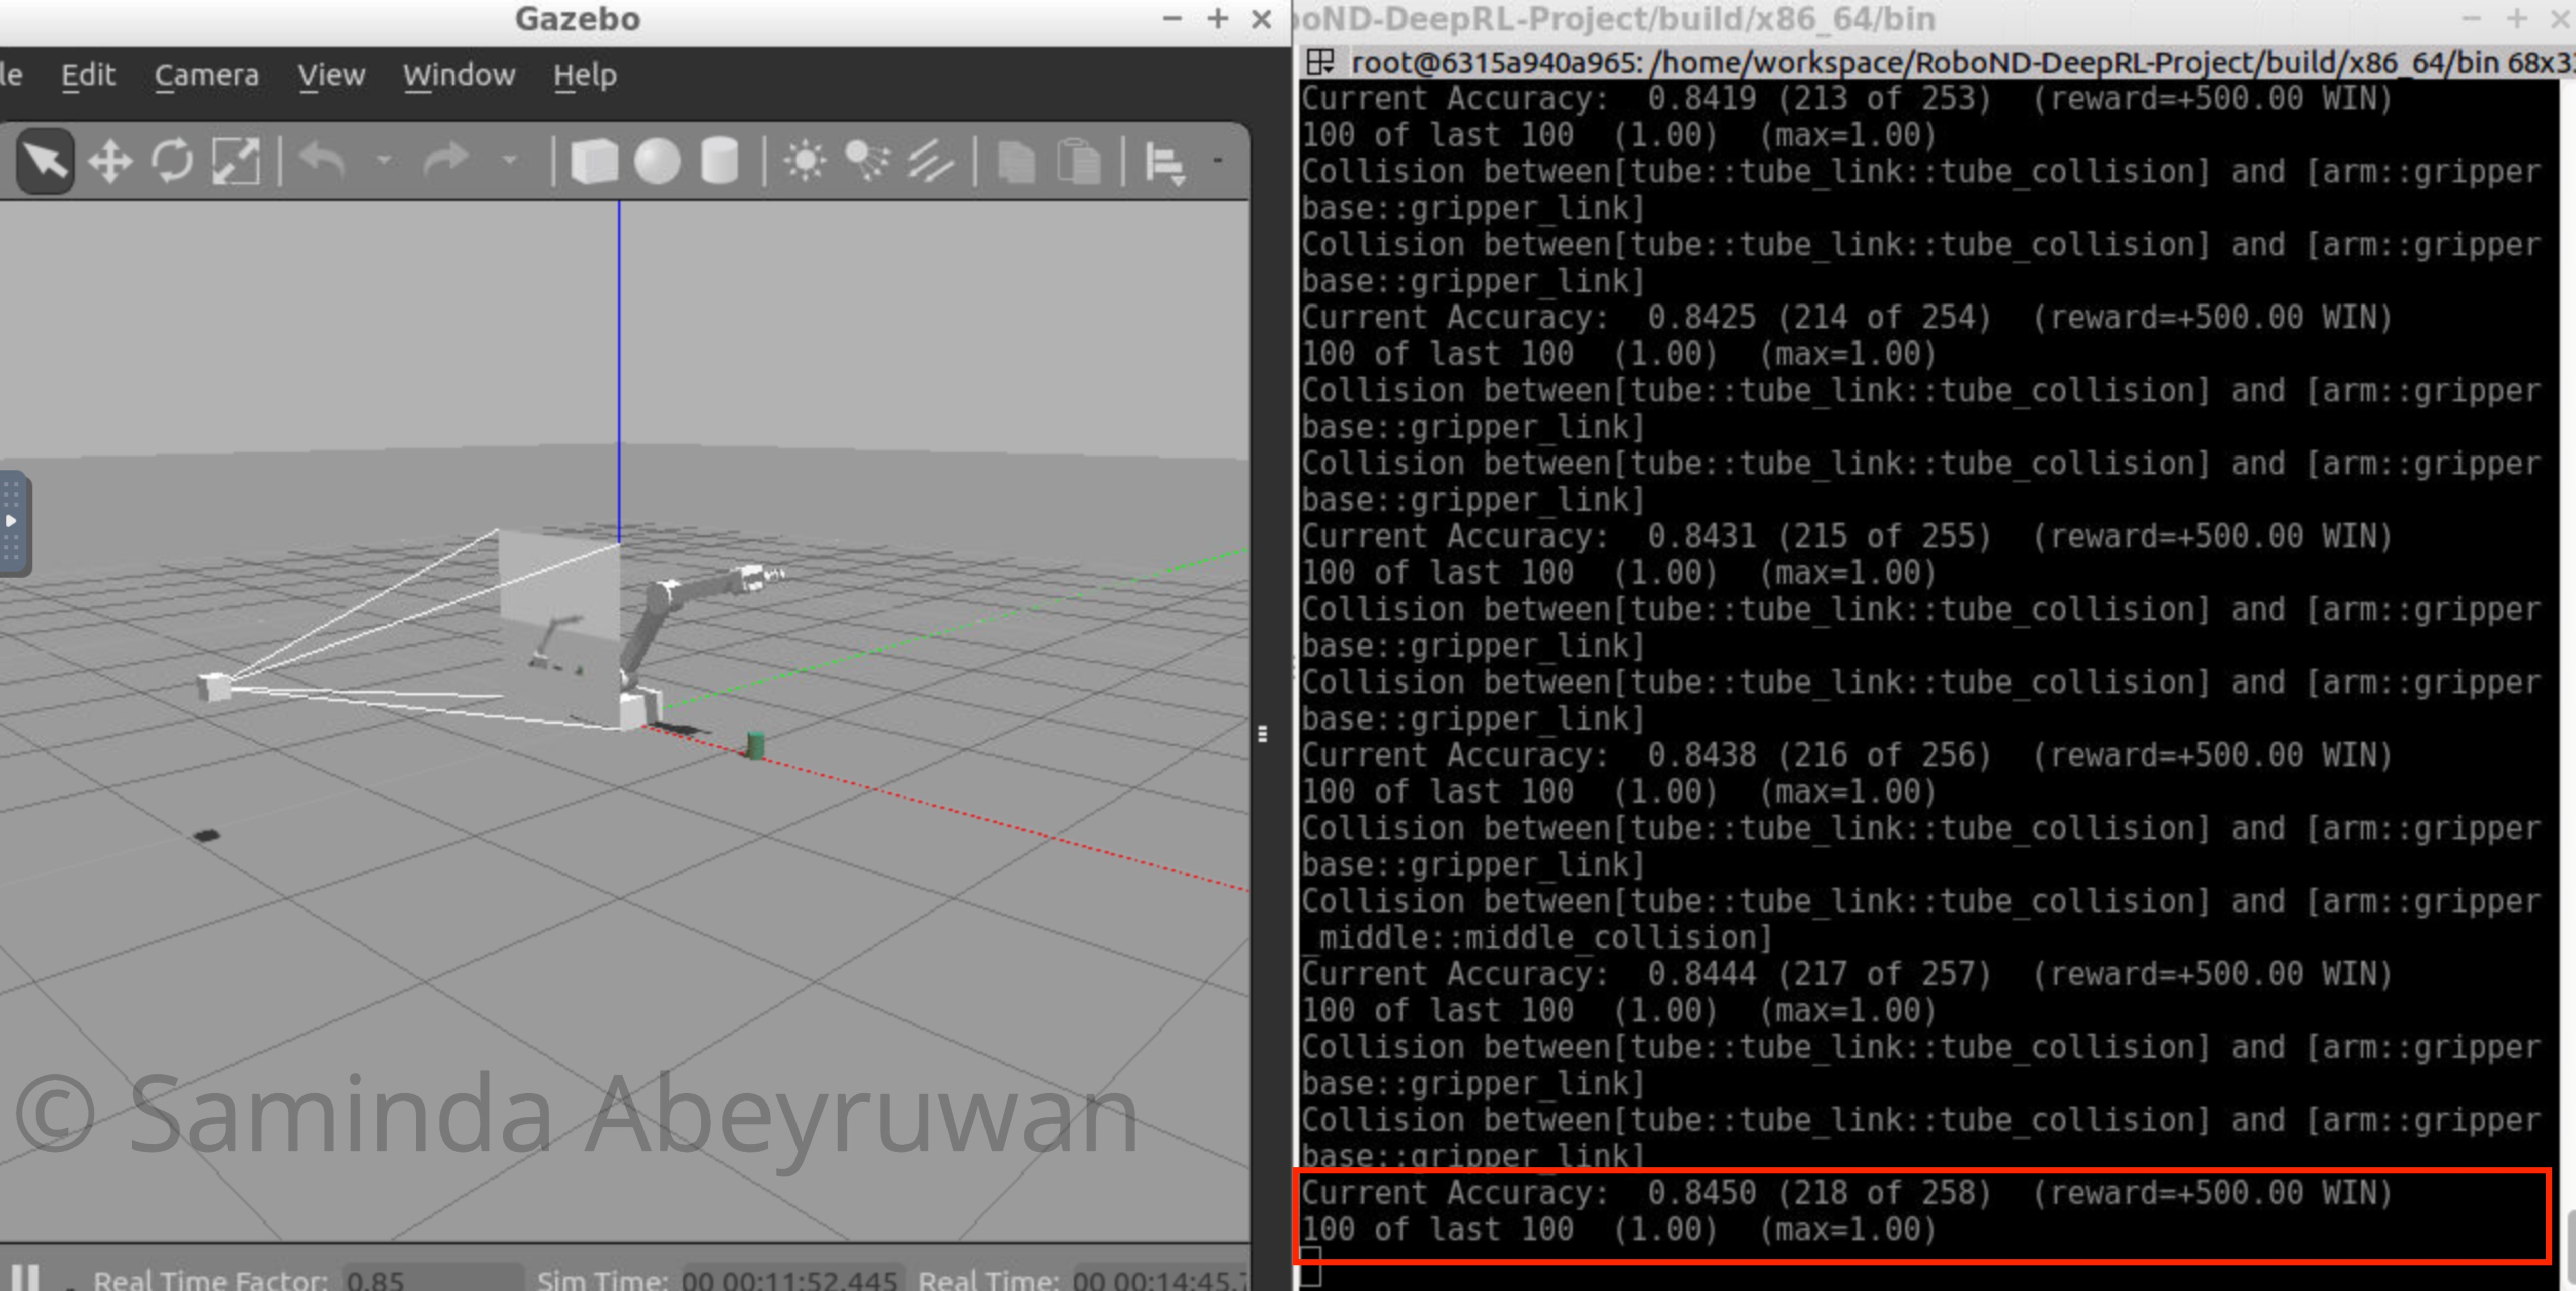
\includegraphics[width=\linewidth]{task1}
      \caption{Task 1: have any part of the robot arm touch the object of interest.}
      \label{fig:task1}
\end{figure*}

\begin{figure*}[thpb]
      \centering
      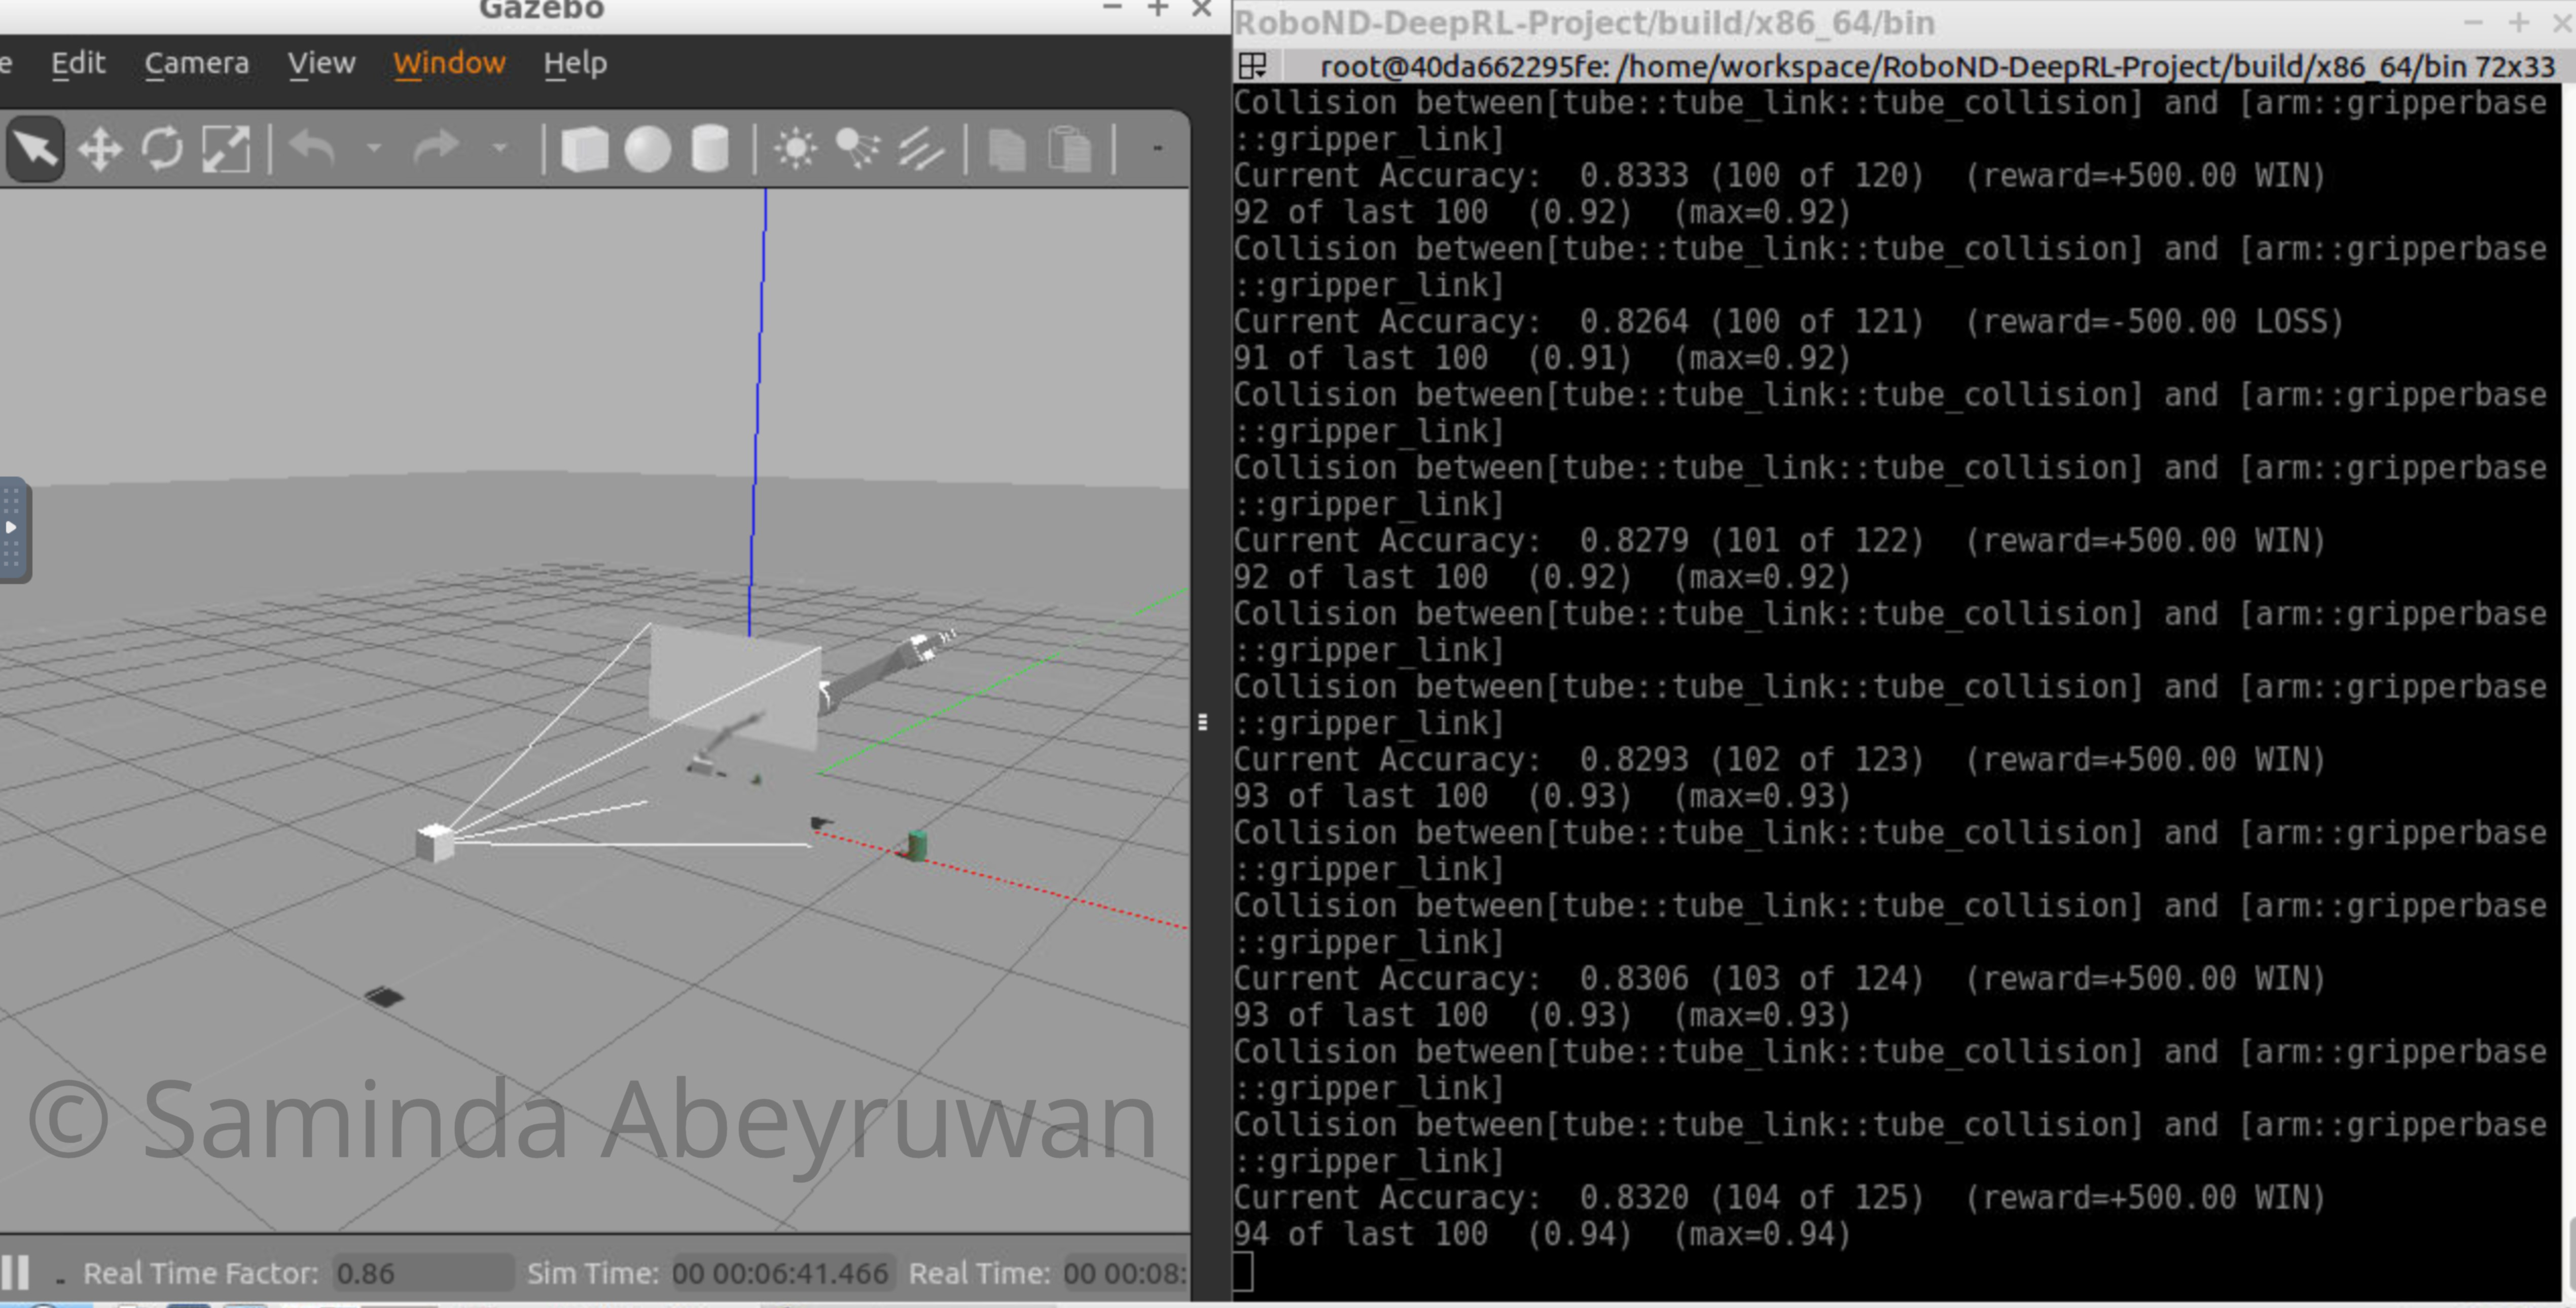
\includegraphics[width=\linewidth]{task2}
      \caption{Task 2: have only the gripper base of the robot arm touch the object.}
      \label{fig:task2}
\end{figure*}


\section{Conclusion / Future work}

In this project, we have trained 3 DoF robotic arm to successfully complete two tasks in simulation using  LSTM based deep-\textit{Q}-networks. A generalized set up based on the current project would help to train other robotic problems. Even though we have used position control, a more realistic robotic control is based on velocity control, which requires continuous control for best performance. The algorithms such as Deep Deterministic Policy Gradient (DDPG), and Normalized Advantage Function algorithm (NAF)  \cite{GuHolLilLev17} have shown state-of-the-art results, and will be benefited to the tasks presented in this project to obtain more realistic results. 

%This section is intended to summarize your report. Your summary should include a recap of the results, did this project achieve what you attempted, and is this a commercially viable product? 
%For Future work,address areas of work that you may not have addressed in your report as possible next steps. For future work, this could be due to time constraints, lack of currently developed methods / technology, and areas of application outside of your current implementation. Again, avoid the use of the first-person.

\bibliography{bib}
\bibliographystyle{ieeetr}

\end{document}